\documentclass[11pt,a4paper]{article}
\usepackage[margin=2.3cm]{geometry}
\usepackage{amsmath,amssymb,amsthm,bm}
\usepackage{booktabs,longtable,array,tabularx}
\usepackage{graphicx}
\usepackage[hidelinks]{hyperref}
\usepackage{enumitem}
\usepackage{xcolor}
\usepackage{tikz}
\usetikzlibrary{arrows.meta,positioning}
\setlist{itemsep=2pt,topsep=4pt}
\usepackage{microtype}
\setlength{\emergencystretch}{3em}
\newcommand{\code}[1]{\texttt{\detokenize{#1}}}
\newcommand{\R}{\mathbb{R}}
\newcommand{\E}{\mathbb{E}}
\DeclareMathOperator{\sign}{sign}
\DeclareMathOperator{\clip}{clip}
\DeclareMathOperator{\diag}{diag}
\newtheorem{proposition}{Proposition}
\input{build/facts.tex}
\makeatletter\newcommand{\rows}[1]{\@@input #1 }\makeatother  % table rows from a file (expandable \input)

\title{News-Driven Risk Budgeting\\[4pt]\large From financial news to portfolio weights}
\author{nabia --- \code{python/} project}
\date{Results as of \WeightDate}

\begin{document}
\maketitle

\begin{abstract}
This document describes the pipeline of the \code{python/} folder, step by step and with its mathematics. Financial
news is collected into a SQLite database and scored by a language model on 27 economic factors. The portfolio's
assets are mapped to those factors by estimating, from price data, how each asset moves with each factor. The
factor sentiment, carried through those exposures, scales each asset's risk budget, and the nabia risk budgeting
optimizer (C++) turns the budgets into long-only weights. Every step is point in time: at a date $t$ it only uses
information available before $t$. The database currently holds \NewsCount{} articles (\NewsFirst{} to \NewsLast{}),
of which \ScoredCount{} have been scored so far.
\end{abstract}

\tableofcontents

%======================================================================
\section{Overview}

\begin{figure}[h]
\centering
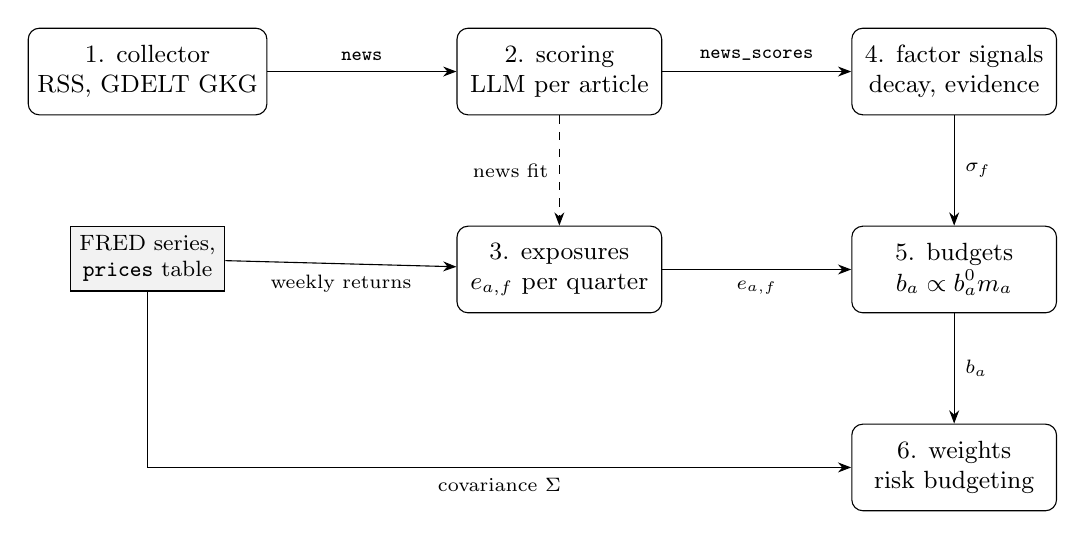
\begin{tikzpicture}[node distance=9mm and 24mm, box/.style={draw, rounded corners, align=center, minimum width=26mm,
  minimum height=11mm, font=\small}, data/.style={draw, fill=gray!10, align=center, font=\footnotesize},
  lab/.style={font=\scriptsize, fill=white, inner sep=1pt}, >={Stealth}]
\node[box] (collect) {1. collector\\RSS, GDELT GKG};
\node[box, right=of collect] (score) {2. scoring\\LLM per article};
\node[box, right=of score] (signal) {4. factor signals\\decay, evidence};
\node[box, below=14mm of signal] (budget) {5. budgets\\$b_a \propto b^0_a m_a$};
\node[box, below=14mm of score] (expo) {3. exposures\\$e_{a,f}$ per quarter};
\node[box, below=14mm of budget] (weights) {6. weights\\risk budgeting};
\node[data, below=14mm of collect] (fred) {FRED series,\\\code{prices} table};
\draw[->] (collect) -- node[lab, above=1mm]{\code{news}} (score);
\draw[->] (score) -- node[lab, above=1mm]{\code{news_scores}} (signal);
\draw[->] (signal) -- node[lab, right=1mm]{$\sigma_f$} (budget);
\draw[->] (fred) -- node[lab, below=1mm]{weekly returns} (expo);
\draw[->] (expo) -- node[lab, below=1mm]{$e_{a,f}$} (budget);
\draw[->, dashed] (score) -- node[lab, left=1mm]{news fit} (expo);
\draw[->] (budget) -- node[lab, right=1mm]{$b_a$} (weights);
\draw[->] (fred.south) |- node[lab, pos=0.75, below=1mm]{covariance $\Sigma$} (weights.west);
\end{tikzpicture}
\caption{The six steps and the database tables between them.}
\end{figure}

\begin{enumerate}
\item \textbf{Collection} (\code{collector/}): RSS feeds (today's items) and GDELT GKG files (history) are stored in
  the \code{news} table, with duplicates removed.
\item \textbf{Scoring} (\code{scoring/}): one language-model call per article gives a sentiment
  $s\in[-1,1]$ and a confidence $c\in[0,1]$ for each factor the article concerns (\code{news_scores}).
\item \textbf{Exposures} (\code{exposures/}): every quarter, a rolling regression of each asset's weekly returns on
  orthogonalized factor proxies (and on the factors' news) gives the signed exposure $e_{a,f}\in[-1,1]$
  (\code{asset_exposures}).
\item \textbf{Factor signals} (\code{budgets/compute.py}): the scores are aggregated per factor into a decayed,
  evidence-weighted signal $\sigma_f(t)\in[-1,1]$.
\item \textbf{Risk budgets}: the asset score $S_a(t)=\sum_f e_{a,f}\sigma_f(t)/\sum_f|e_{a,f}|$ scales the base
  budget, $b_a\propto b^0_a\,(1+\kappa S_a)$ (\code{risk_budgets}).
\item \textbf{Weights} (\code{budgets/weights.py}): the long-only weights whose risk contributions equal the
  budgets, from the C++ optimizer of \code{nabia_python_bridge} (\code{portfolio_weights}).
\end{enumerate}

All settings are in \code{config/config.json}; the factors are in \code{config/factors.json}. Section~\ref{sec:run}
shows how to run each step.

%======================================================================
\section{Data layer}

All data is in \code{data/market.db} (SQLite), read and written through the \code{datalayer} package:
\code{NewsDB} for the news tables, \code{MarketDB} for the market tables. Times are UTC ISO~8601 strings, so they sort
and compare as text.

\begin{center}
\begin{tabularx}{\linewidth}{@{}l l X@{}}
\toprule
table & one row per & content \\
\midrule
\code{prices} & symbol $\times$ day & daily OHLC and adjusted close of the assets and price proxies (pre-existing) \\
\code{assets} & symbol & name, asset class, currency (pre-existing; referenced by \code{prices}) \\
\code{news} & article & url, headline, body, source, \code{published_at}, \code{received_at}, \code{dedup_key} \\
\code{news_scoring} & article $\times$ model $\times$ prompt & relevant flag, scoring time \\
\code{news_scores} & article $\times$ model $\times$ prompt $\times$ factor & sentiment $s$, confidence $c$ \\
\code{series} & series $\times$ day & downloaded FRED series (key \code{fred:<id>}) \\
\code{asset_exposures} & quarter end $\times$ asset $\times$ factor & $e_{a,f}$, raw beta, $t$-statistic, stability, method \\
\code{risk_budgets} & rebalance $\times$ asset & base budget, score $S_a$, multiplier $m_a$, budget $b_a$ \\
\code{portfolio_weights} & rebalance $\times$ asset & budget, weight $w_a$, risk contribution, portfolio risk \\
\bottomrule
\end{tabularx}
\end{center}

%======================================================================
\section{News collection}

\paragraph{Sources.}
\begin{itemize}
\item \textbf{RSS and Atom feeds} (\code{collect.feeds}: MarketWatch, CNBC, Financial Times, Investing.com, OilPrice,
  Federal Reserve, ECB, Bank of England). Feeds carry no history, so they only give today's items;
  \code{received_at} is the download time.
\item \textbf{GDELT Global Knowledge Graph.} Every 15 minutes GDELT publishes a file listing the web articles it has
  processed, with their page titles. For each weekday since \code{collect.since}, two 15-minute slices
  (14:30 and 20:30 UTC) are read, the titles matching a finance and macro vocabulary are kept, well-known financial
  outlets are ranked first, and at most \code{gkg_per_day} = 10 articles are stored. \code{received_at} is the GKG
  timestamp: when GDELT processed the article, a point-in-time stamp. GKG gives titles only, so the body is the
  headline.
\end{itemize}
Each run continues GKG from the day after the last GKG day stored. \code{--since} collects from a given day, and
\code{--import} loads a \code{news.json} file of the former project.

\paragraph{Deduplication.} With $\nu(h)$ the headline lower-cased and reduced to its alphanumeric words, an article
is stored only if both its URL and its key
\[
  k = \nu(\text{headline}) \,\|\, \text{day}(\text{received\_at})
\]
are new (\code{UNIQUE} constraints and \code{INSERT OR IGNORE}). The same story syndicated by several outlets on the
same day is therefore stored once.

%======================================================================
\section{Economic factors}

\code{config/factors.json} lists 27 factors. The sign convention is the same for all of them:
\begin{center}
\fbox{\parbox{0.86\linewidth}{\centering $s>0$ means \emph{the factor itself goes up}: more growth, more inflation,
tighter policy, wider spreads, more stress, more conflict, a stronger currency, whether or not that is good news for
markets.}}
\end{center}
This makes the sign independent of the asset. Whether a move of the factor is good or bad for an asset is learned
from data in the exposure step (Section~\ref{sec:exposures}). Each factor has a \code{group} and a \code{region} tag,
used for shrinkage and fallbacks. There is no tree: the drivers cut across asset classes (the Fed moves equities,
bonds, gold and the dollar at once), so a hierarchy would force a single parent per node and make features
collinear. Table~\ref{tab:factors} lists them, with the method that produced their current exposures.

{\footnotesize
\begin{longtable}{@{}p{3.6cm} p{1.6cm} p{1.4cm} p{1.1cm} p{6.6cm}@{}}
\caption{The factors, their tags and the method of their latest exposures (\code{proxy}: market proxy;
\code{group}: borrowed from the group; \code{none}: no information yet).}\label{tab:factors}\\
\toprule factor & group & region & method & sentiment $>0$ means \\ \midrule \endfirsthead
\toprule factor & group & region & method & sentiment $>0$ means \\ \midrule \endhead
\rows{build/methods.tex}
\bottomrule
\end{longtable}}

%======================================================================
\section{Scoring with a language model}

\subsection{The call}
Each article gets one call. The \emph{system prompt} holds the instructions, the sign rule, the scale and the factor
list (\code{id | name | positive meaning}); it is identical for every article, so a local model reuses its processed
prefix and an API can cache it. The \emph{user prompt} holds only the article: timestamp, source, headline and body
(truncated to 4000 characters). The answer is constrained to the JSON schema
\[
  \{\ \code{relevant}: \text{bool},\ \ \code{scores}: [\,\{\code{factor} \in \mathcal F,\ \code{sentiment},\ \code{confidence}\}\,]\ \}
\]
through the provider's structured output: Ollama's \code{format}, OpenAI's \code{json_schema} (strict) or an
Anthropic tool whose input is the schema. Temperature is 0.

The scale given to the model is $\pm1$ for a major, unambiguous move, $\pm0.5$ for a clear moderate one, $\pm0.2$ for
a mild one and $0$ for neutral or in-line news. The rules: use only the article; score the news against the
expectations it states; reported price moves are reactions, not information; usually one to three factors; lower
confidence for rumours, opinion and headline-only items.

\subsection{Validation}
For an answer with entries $(f_j, s_j, c_j)$, unknown factors are dropped, one entry per factor is kept, and values
are clipped:
\[
  s \leftarrow \clip(s, -1, 1), \qquad c \leftarrow \clip(c, 0, 1).
\]
The article is \emph{relevant} if the model says so and at least one valid score remains. A malformed answer or a
network error is retried up to \code{llm.max_retries} times; an article still failing is skipped and retried on the
next run.

\subsection{Versions and resumption}
The prompt version is $v = \mathrm{SHA256}(\text{system prompt} \,\|\, \text{user template})_{1..12}$. Since the
system prompt contains the factor list, editing either the prompt or the factors changes $v$. A scoring is stored
per (article, model, $v$), and only articles without a scoring for the current model and version are sent, so an
interrupted run resumes where it stopped and a new version rescores everything, keeping the old scores.

\subsection{Providers and throughput}
\code{llm.provider} selects a local Ollama model (\code{gemma4:26b}, the default; about 5\,s per article), the OpenAI
Chat Completions API or the Anthropic Messages API, with the key read from the environment variable named in the
configuration. \code{llm.workers} requests run in parallel threads (database writes stay in the main thread); HTTP 429
and 5xx answers are retried after the server's \code{Retry-After}, and \code{llm.requests_per_minute} spaces the
request starts across workers. \code{--dry-run} reports the number of articles and their prompt tokens before an API
run.

%======================================================================
\section{Asset exposures}\label{sec:exposures}

The exposure $e_{a,f}$ answers: \emph{when factor $f$ moves up, how does asset $a$ move?} It is estimated from
prices, which have a long history, rather than from the news, which is short.

\subsection{Weekly returns}
Every daily series $X$ is sampled at the last observation of each week (Friday), $X_\tau$, and transformed into a
weekly change:
\[
  \Delta_\tau X = \begin{cases} \ln X_\tau - \ln X_{\tau-1} & \text{prices, indices, FX, VIX (\code{logret})},\\
  X_\tau - X_{\tau-1} & \text{yields, spreads, stress indices (\code{diff})}. \end{cases}
\]
Weekly returns avoid the bias of daily returns between markets closing at different hours (Tokyo, Hong Kong,
Europe, New York). The proxy of factor $f$ is a weighted sum of terms $(X_j, \text{transform}_j, \omega_j)$ from
\code{factors.json}:
\[
  p_{f,\tau} = \sum_j \omega_j \,\Delta_\tau X_j .
\]

\begin{center}\small
\begin{tabularx}{\linewidth}{@{}l X l@{}}
\toprule
factor & proxy $p_f$ & source \\
\midrule
GROWTH\_US & $\Delta\ln$ Russell 2000 & \code{prices} \\
GROWTH\_EUROPE & $\Delta\ln$ Euro Stoxx 50 & \code{prices} \\
GROWTH\_CHINA & $\Delta\ln$ Hang Seng & \code{prices} \\
TECH\_AI & $\Delta\ln$ Nasdaq 100 $-$ $\Delta\ln$ S\&P 500 & \code{prices} \\
POLICY\_FED & $\Delta$ 2-year Treasury yield (\code{DGS2}) & FRED \\
FISCAL\_US & $\Delta$ 10-year term premium (\code{THREEFYTP10}) & FRED \\
ENERGY\_SUPPLY & $\Delta\ln$ Brent future & \code{prices} \\
INDUSTRIAL\_METALS & $\Delta\ln$ copper future & \code{prices} \\
AGRICULTURE & $\tfrac13(\Delta\ln$ corn $+$ soy $+$ wheat futures$)$ & \code{prices} \\
INFLATION\_US & $\Delta$ 10-year breakeven inflation (\code{T10YIE}) & FRED \\
CREDIT\_STRESS & $\Delta$ Baa $-$ 10-year spread (\code{BAA10Y}) & FRED \\
BANKING\_STRESS & $\Delta$ St.\ Louis Fed financial stress index (\code{STLFSI4}) & FRED \\
RISK\_APPETITE & $-\Delta\ln$ VIX (\code{VIXCLS}) & FRED \\
USD & $\Delta\ln$ broad dollar index (\code{DTWEXBGS}) & FRED \\
JPY & $-\Delta\ln$ yen per dollar (\code{DEXJPUS}) & FRED \\
CNY & $-\Delta\ln$ yuan per dollar (\code{DEXCHUS}) & FRED \\
GOLD\_DEMAND & $\Delta\ln$ gold future & \code{prices} \\
\bottomrule
\end{tabularx}
\end{center}
The HY option-adjusted spread is no longer distributed by FRED beyond three years, hence the Baa spread. Ten factors
have no market proxy (the non-Fed central banks, European sovereign risk and inflation, emerging-market growth,
earnings, geopolitics, trade policy).

\subsection{Orthogonalization}
At each quarter end $q$, take the last $T=156$ weeks (\code{window_weeks}). Proxies with less than 90\% of the weeks
are left out, and weeks with any missing value are dropped. Let $P\in\R^{T\times K}$ hold the proxies in the order of
\code{factors.json}, $X = P - \bar P$ its centred columns and $y\in\R^T$ the asset's centred weekly log returns.
Proxies are correlated (equities and the 2-year yield, Brent and growth), so they are made orthogonal in that order,
with the QR decomposition
\[
  X = QR, \qquad Q^\top Q = I_K, \quad R \text{ upper triangular}.
\]
\begin{proposition}
The $k$-th column of $Q R_{kk}$ (with $R_{kk}$ the diagonal entry) is the residual $z_k$ of the regression of $x_k$ on
$x_1,\dots,x_{k-1}$: proxy $k$ net of the proxies before it. The residuals are mutually orthogonal and
$\|z_k\| = |R_{kk}|$.
\end{proposition}
\begin{proof}
$x_k = \sum_{j\le k} R_{jk} q_j$, and $q_1,\dots,q_{k-1}$ span the same space as $x_1,\dots,x_{k-1}$. The projection of
$x_k$ on that space is $\sum_{j<k}R_{jk}q_j$, so the residual is $R_{kk}q_k$, orthogonal to the earlier columns and to
the other $q_j$.
\end{proof}
The order is an \emph{identification assumption}: the variance two proxies share is attributed to the earlier one.
The file puts equity growth first, so the 2-year yield net of equities is read as a monetary-policy shock; Brent net
of growth as an energy-supply shock; breakevens net of growth and energy as inflation; gold last, net of the dollar
and the Fed.

\subsection{Exposures and \texorpdfstring{$t$}{t}-statistics}
Regressing $y$ on the orthogonal residuals $z_1,\dots,z_K$ gives, column by column,
\[
  \beta_k = \frac{z_k^\top y}{z_k^\top z_k} = \frac{q_k^\top y}{R_{kk}},
  \qquad
  \hat\varepsilon = y - Q Q^\top y, \qquad \hat\sigma^2 = \frac{\|\hat\varepsilon\|^2}{T-K-1}.
\]
The exposure is the standardized coefficient and the $t$-statistic uses $\operatorname{se}(\beta_k)=\hat\sigma/\|z_k\|$:
\[
  \boxed{\;e^{\text{raw}}_{a,k} = \beta_k\frac{\|z_k\|}{\|y\|} = \sign(R_{kk})\,\frac{q_k^\top y}{\|y\|},
  \qquad t_{a,k} = \frac{\beta_k}{\operatorname{se}(\beta_k)} = \sign(R_{kk})\,\frac{q_k^\top y}{\hat\sigma}.\;}
\]
$e^{\text{raw}}_{a,k}$ is the correlation of the asset with the factor's shock, in $[-1,1]$, and since the $q_k$ are
orthonormal,
\[
  \sum_k \big(e^{\text{raw}}_{a,k}\big)^2 = \frac{\|QQ^\top y\|^2}{\|y\|^2} = R^2_a ,
\]
so the squared exposures split the share of the asset's weekly variance that the factors explain.

\subsection{News fit}
For a factor with news, its weekly sentiment is the confidence-weighted mean of the scores of the articles received
that week, an article scored by several models or prompt versions counting once with its mean score:
\[
  \bar s_{f,\tau} = \frac{\sum_{i\in\tau} c_{i,f}\, s_{i,f}}{\sum_{i\in\tau} c_{i,f}} .
\]
If at least $n_{\min}=52$ weeks of the window have news (\code{news_min_weeks}), the news fit is the correlation
$r$ between $\bar s_{f,\cdot}$ and the asset's returns over those $n$ weeks, with
$t = r\sqrt{(n-2)/(1-r^2)}$. It fills the factors without a proxy and, with \code{news_override}, replaces the proxy
fit when $|t|\ge t_{\min}$: news captures what a proxy cannot, such as a Fed shock on equities, which the ordering
above assigns to growth.

\subsection{Selection, shrinkage and fallback}
For asset $a$ at quarter $q$, with fits $(e^{\text{raw}}_{a,f}, t_{a,f})$ by method $\mu\in\{\text{proxy},\text{news}\}$:
\begin{enumerate}
\item \textbf{Significance and stability.} With $\mathcal H$ the last $8$ fits of the same pair and method
  (\code{stability_windows}), the stability is
  \[
    \pi_{a,f} = \frac{1}{|\mathcal H|}\sum_{h\in\mathcal H} \mathbf 1\big[\sign e_h = \sign e^{\text{raw}}_{a,f}\big],
  \]
  and the exposure is kept only if it is significant and stable:
  \[
    \tilde e_{a,f} = e^{\text{raw}}_{a,f}\;\mathbf 1\big[\,|t_{a,f}|\ge t_{\min}\ \wedge\ \pi_{a,f}\ge \pi_{\min}\big],
    \qquad t_{\min}=2,\ \pi_{\min}=0.75 .
  \]
\item \textbf{Shrinkage toward the group.} With $G(f)$ the fitted factors of $f$'s group and
  $\bar e_{a,G} = \frac1{|G|}\sum_{g\in G}\tilde e_{a,g}$,
  \[
    e_{a,f} = (1-\lambda)\,\tilde e_{a,f} + \lambda\,\bar e_{a,G(f)}, \qquad \lambda = 0.25 \ (\code{group_shrink}).
  \]
\item \textbf{Fallback.} A factor without a fit borrows $e_{a,f} = \gamma\,\bar e_{a,G(f)}$ with $\gamma=0.5$
  (\code{group_fallback}); if its group has no fit, $e_{a,f}=0$.
\end{enumerate}
Each $(q, a, f)$ is stored with $e$, $e^{\text{raw}}$, $t$, $\pi$ and the method. \code{MarketDB.exposures(t)} returns
the map of the latest quarter end before $t$, so a backtest only uses exposures that were known.

\subsection{Results}
Figure~\ref{fig:exposures} shows the map at \ExposureDate{} (of \ExposureDates{} quarter ends since 2012). The
structure is economically sensible: bonds load on the Fed in order of duration sensitivity to short rates (2-year
$-0.94$, 10-year $-0.86$, 30-year $-0.73$) and the 30-year on fiscal supply ($-0.57$); equities on growth and the AI
cycle; each commodity on its own supply factor; gold also negatively on the dollar and the Fed. The non-Fed central
banks show half of the Fed's exposures (fallback) until their news fit becomes available. Figure~\ref{fig:history}
shows how some exposures moved over time.

\begin{figure}[p]
\centering\includegraphics[width=\linewidth]{build/exposures.pdf}
\caption{Exposures $e_{a,f}$ at \ExposureDate. Blank cells are zero: not significant, not stable, or no information.}
\label{fig:exposures}
\end{figure}

\begin{figure}[t]
\centering\includegraphics[width=\linewidth]{build/exposure_history.pdf}
\caption{Exposure history of selected asset--factor pairs (zero when the tests fail).}
\label{fig:history}
\end{figure}

%======================================================================
\section{Factor signals}

At a rebalance date $t$, the signal of factor $f$ uses the articles received strictly before day $t$. With
$d_i$ the receipt day of article $i$, its age $\Delta_i = t - d_i \ge 1$ days, the half-life $H$
(\code{half_life_days} $=5$) and $\delta = 2^{-1/H}$, the decayed sums are
\[
  N_f(t) = \sum_{i:\, d_i < t} \delta^{\,\Delta_i - 1}\, c_{i,f}\, s_{i,f},
  \qquad
  D_f(t) = \sum_{i:\, d_i < t} \delta^{\,\Delta_i - 1}\, c_{i,f}.
\]
They are computed recursively over calendar days, $N(t) = \delta N(t-1) + \sum_{i: d_i = t-1} c_i s_i$ (and the
same for $D$). The level is the decayed, confidence-weighted mean sentiment, and the signal shrinks it by the amount
of evidence:
\[
  \ell_f(t) = \frac{N_f(t)}{D_f(t)} \in [-1,1],
  \qquad
  \boxed{\;\sigma_f(t) = \ell_f(t)\,\frac{D_f(t)}{D_f(t) + \eta}\;}
  \qquad \eta = 3\ (\code{evidence}),
\]
with $\sigma_f = 0$ when $D_f = 0$. $D_f$ counts the recent articles, weighted by confidence and age: a factor with one
confident article from yesterday has $D_f\approx1$ and keeps a quarter of its level; with twelve, $D_f\approx 12$ and
it keeps 80\%. The sign of $\sigma_f$ follows the factor convention: $\sigma_f>0$ means the news says the factor is
going up.

%======================================================================
\section{Risk budgets}

\subsection{Asset score}
With $e_{a,f}$ the latest exposure map estimated before $t$,
\[
  \boxed{\;S_a(t) = \frac{\sum_f e_{a,f}\,\sigma_f(t)}{\sum_f |e_{a,f}|}\;} \in [-1,1],
\]
with $S_a = 0$ for an asset without exposures. It is the exposure-weighted average of the factor signals, each signed
by how the asset responds: hawkish Fed news ($\sigma_{\text{FED}}>0$) times the 2-year note's
$e=-0.94$ lowers the note's score; energy-supply news lifts Brent's. $S_a>0$ means the news is bullish for the asset.
The contribution of factor $f$, $e_{a,f}\sigma_f/\sum_g|e_{a,g}|$, is printed by the command line, so every budget
change can be traced to its news.

\subsection{Budgets}
With base budgets $b^0_a$ (\code{budgets.base}, equal when null), strength $\kappa = 0.5$ and bounds
$[m_{\min}, m_{\max}] = [0.5, 1.5]$:
\[
  m_a(t) = \clip\big(1 + \kappa\, S_a(t),\ m_{\min},\ m_{\max}\big),
  \qquad
  \boxed{\;b_a(t) = \frac{b^0_a\, m_a(t)}{\sum_j b^0_j\, m_j(t)}\;}.
\]
Budgets stay positive (the optimizer needs $b_a>0$) and sum to one. With $|S_a|\le1$ and $\kappa=0.5$, an asset's
budget can at most be multiplied by $1.5$ or halved relative to the others. Budgets are computed every Friday
(\code{budgets.frequency}) since \code{budgets.start}.

%======================================================================
\section{Weights by risk budgeting}

\subsection{Covariance}
At rebalance $t$, $\Sigma$ is the sample covariance of the assets' weekly simple returns over the last $104$ weeks up
to $t$ (\code{cov_window_weeks}), annualized ($\times52$) and shrunk toward its diagonal:
\[
  \Sigma = (1-\rho)\,\hat\Sigma + \rho\,\diag(\hat\Sigma), \qquad \rho = 0.1\ (\code{shrinkage}).
\]
The shrinkage keeps $\Sigma$ well conditioned with 13 assets and 104 observations; at least 80\% of the window must
have complete data.

\subsection{The risk budgeting problem}
For a risk measure $\mathcal R(w)$ that is convex and positively homogeneous of degree one, Euler's theorem gives
$\mathcal R(w) = \sum_a w_a\,\partial_a \mathcal R(w)$, and the \emph{risk contribution} of asset $a$ is
$RC_a = w_a\,\partial_a\mathcal R(w)$. With the volatility (\code{risk_measure} = \code{Volatility}),
\[
  \mathcal R(w) = \sqrt{w^\top\Sigma w}, \qquad RC_a = \frac{w_a (\Sigma w)_a}{\sqrt{w^\top \Sigma w}} .
\]
The risk budgeting portfolio is the long-only, fully invested $w$ whose relative contributions equal the budgets:
\[
  w_a > 0, \quad \sum_a w_a = 1, \quad \frac{RC_a(w)}{\mathcal R(w)} = b_a \quad \forall a .
\]
\begin{proposition}[Roncalli; Spinu]
Let $y^\star$ solve the strictly convex problem
\[
  \min_{y>0}\ F(y) = \mathcal R(y) - \sum_a b_a \ln y_a .
\]
Then $w = y^\star/\sum_a y^\star_a$ is the unique risk budgeting portfolio.
\end{proposition}
\begin{proof}
The first-order condition is $\partial_a\mathcal R(y) = b_a/y_a$, i.e.\ $y_a\partial_a\mathcal R(y) = b_a$: the risk
contributions of $y$ are the budgets, and $\mathcal R(y)=\sum_a b_a = 1$. Since $\partial_a\mathcal R$ is homogeneous
of degree zero, $w=y/\sum y$ has $RC_a(w)/\mathcal R(w) = RC_a(y)/\mathcal R(y) = b_a$. $F$ is strictly convex (convex
$\mathcal R$ plus a strictly convex barrier) and tends to $+\infty$ at the boundary and at infinity, so the minimizer
exists and is unique.
\end{proof}
The C++ implementation (\code{nabia::risk::RiskBudgeting}) minimizes $F$ with L-BFGS; the log barrier keeps $y>0$
(the line search rejects steps leaving the domain). It stops when $\max_a |RC_a/\mathcal R - b_a|$ is below the
tolerance ($10^{-10}$ here). Each rebalance starts from the previous weights, which are close to the solution. The
Gaussian Value-at-Risk and Expected Shortfall can be used instead (\code{risk_measure}):
\[
  \mathrm{VaR}_\alpha(w) = z_\alpha\sqrt{w^\top\Sigma w}, \qquad
  \mathrm{ES}_\alpha(w) = \frac{\phi(z_\alpha)}{1-\alpha}\sqrt{w^\top\Sigma w}, \qquad z_\alpha = \Phi^{-1}(\alpha),
\]
which, without expected returns, are multiples of the volatility and give the same weights.

\subsection{Results}
All \Rebalances{} weekly rebalances converged, with every risk contribution equal to its budget. Since only
\ScoredCount{} articles are scored, all received after the last rebalance, the budgets are still equal and the
portfolio is the equal risk contribution portfolio. Its annualized volatility is \PortfolioRisk{}
(Table~\ref{tab:weights}). The 2-year note receives most of the capital because its volatility is a fraction of the
others': equal risk needs inverse-volatility-like weights. A portfolio with a volatility target would lever it up.

\begin{table}[h]
\centering\small
\begin{tabular}{@{}l r r r@{}}
\toprule asset & budget $b_a$ & weight $w_a$ & risk contribution $RC_a/\mathcal R$ \\ \midrule
\rows{build/weights.tex}
\bottomrule
\end{tabular}
\caption{Budgets, weights and risk contributions at \WeightDate.}\label{tab:weights}
\end{table}

\begin{figure}[h]
\centering\includegraphics[width=\linewidth]{build/weights.pdf}
\caption{Weights at each weekly rebalance.}
\end{figure}

%======================================================================
\section{Point in time}
Every step only uses what was known at the date it computes:
\begin{itemize}
\item \code{received_at} is the time an article became available (download time, GKG processing time), not the
  publication time an outlet may backdate.
\item The factor signal at $t$ uses articles received before day $t$; the budgets at $t$ use the exposure map of the
  latest quarter end before $t$.
\item Each exposure uses returns up to its quarter end only; its stability test uses earlier quarters only.
\item The covariance at $t$ uses returns up to $t$.
\end{itemize}
Two things are not point in time: the language model knows what happened after the articles it scores (the prompt
forbids using that knowledge, but this cannot be guaranteed), and FRED series can be revised after their release.

%======================================================================
\section{Running the pipeline}\label{sec:run}
From \code{python/}; the first run of \code{run.sh} creates \code{.venv} with numpy, pandas and the
\code{nabia_python_bridge} wheel from \code{../dist}.
\begin{center}\small
\begin{tabular}{@{}l l@{}}
\toprule step & command (\code{py} = \code{.venv/bin/python}) \\ \midrule
all steps & \code{./run.sh [config.json]} \\
1. collect & \code{py -m collector [--since D] [--until D] [--import news.json]} \\
2. score & \code{py -m scoring [--provider P] [--workers N] [--limit N] [--dry-run]} \\
3. exposures & \code{py -m exposures [--no-download]} \\
4--6. budgets, weights & \code{py -m budgets [--start D] [--end D]} \\
tests & \code{py -m unittest discover -s tests} \\
this document & \code{doc/build.sh} \\
\bottomrule
\end{tabular}
\end{center}

\paragraph{Configuration.} The main parameters of \code{config/config.json}:
\begin{center}\small
\begin{tabular}{@{}l l l@{}}
\toprule section & parameters & values \\ \midrule
\code{collect} & \code{since} & 2020-01-01 \\
 & \code{gkg_per_day}, \code{gkg_slices} & 10; 14:30 and 20:30 UTC \\
\code{llm} & \code{provider}, \code{workers}, \code{requests_per_minute} & ollama, 1, none \\
\code{exposures} & \code{window_weeks}, \code{t_min} & 156, 2 \\
 & \code{stability}, \code{stability_windows} & 0.75, 8 \\
 & \code{group_shrink}, \code{group_fallback} & 0.25, 0.5 \\
 & \code{news_min_weeks}, \code{news_override} & 52, true \\
\code{budgets} & \code{half_life_days}, \code{evidence}, \code{strength} & 5, 3, 0.5 \\
 & \code{min_multiplier}, \code{max_multiplier} & 0.5, 1.5 \\
 & \code{frequency} & weekly (Friday) \\
\code{weights} & \code{risk_measure} & Volatility \\
 & \code{cov_window_weeks}, \code{shrinkage} & 104, 0.1 \\
\bottomrule
\end{tabular}
\end{center}

%======================================================================
\section{Limitations and next steps}
\begin{itemize}
\item \textbf{Scoring backlog.} \ScoredCount{} of \NewsCount{} articles are scored. Until the backlog is scored,
  budgets stay at their base and the news fits of the exposures are inactive.
\item \textbf{Identification by ordering.} Equity indices are the growth proxies, so equities get no Fed exposure
  from the proxies; the news fit restores it once enough Fed news is scored. Other orders are possible and change
  the map.
\item \textbf{Headlines only.} GKG gives titles, a weaker signal than full text, and ten articles a day is a thin
  sample per factor.
\item \textbf{Exposure is not prediction.} The exposures measure co-movement. Whether a factor's news \emph{leads}
  returns is not tested here; a backtest of the budgets against equal risk contribution would measure it.
\item \textbf{Futures} are continuous front-month series, so roll jumps add noise to their weekly returns.
\end{itemize}

\end{document}
